\chapter{열역학 제2 법칙과 제3 법칙}
    \section{엔트로피}
        \hspace{\parindent}
        \begin{defn}[엔트로피]
        \textbf{엔트로피(Entropy, $S$)}는 \textit{무질서한 정도를 나타내는 상태 함수로}\footnote[8]{더 정확한 정의는 통계물리학적으로 기술되나, %
        이 노트의 범위를 벗어나므로 생략한다.}, 과정의 자발성을 결정하는 요인이다.
        \end{defn}
        \textbf{열역학 제2 법칙(Second Law of thermodynamics)}은 다음과 같이 두 가지로 
        서술되고, 이 둘은 동치이다:
        \begin{rem}[열역학 제2 법칙의 서술]
        \begin{enum}
            \item Kelvin의 설명: 열을 전부 일로 전환시킬 수는 없다.
            \item Clausius의 설명: 열은 저열원에서 고열원으로 자발적으로 흐를 수 없다. 
        \end{enum}
        \end{rem}
        따라서 엔트로피를 도입할 경우 다음과 같은 설명이 된다.
        \begin{rem}[열역학 제2 법칙의 엔트로피적 서술]
            엔트로피를 도입한 설명: 고립계에서 자발적 반응이 일어날 경우 고립계의 총 엔트로피는 증가한다: $\displaystyle\Delta S_{\mathrm{tot}} > 0$ 
        \end{rem}
        \par 엔트로피 변화의 열역학적 정의는 다음과 같다:
        \begin{defn}[엔트로피 변화]
        가역 과정 중 출입하는 열 $q_{\mathrm{rev}}$에 대해,
        \begin{equation*}
            \difform S = \frac{\difform q_{\mathrm{rev}}}{T}
        \end{equation*}
        따라서 $\displaystyle\Delta S = \int_{i}^{f}\frac{\difform q_{\mathrm{rev}}}{T}$를 만족한다.
        \end{defn}
        단위는 J K$^{-1}$이고, 몰 엔트로피 $S_m = S/n$ 또한 정의할 수 
        있다(단위는 J K$^{-1}$ mol$^{-1}$).
        \par 등온 과정의 엔트로피 변화는 다음과 같이 구할 수 있다: 이때 내부 에너지 변화 $\displaystyle\Delta U = 0$이므로 $q_\mathrm{rev} = -w_\mathrm{rev}$를 이용한다.
        \begin{equation*}
            \begin{aligned}
                \Delta S &= \frac{1}{T}\int_{i}^{f}\difform q_{\mathrm{rev}} = \frac{q_\mathrm{rev}}{T} \\
                &= -\frac{w_{\mathrm{rev}}}{T} = nR \ln{\frac{V_f}{V_i}} \\
                \Delta S_m &= R \ln{\frac{V_f}{V_i}}
            \end{aligned}
        \end{equation*}
        \par 한편, 주위의 엔트로피 변화를 구하기 위해서는 엔트로피의 정의 $\displaystyle\difform S_\mathrm{sur} = \difform q_\mathrm{sur} / T_\mathrm{sur}$를 
        이용한다. 이때 $\displaystyle\difform q_\mathrm{sur} \approx \difform U_{\mathrm{sur}}$로 근사할 수 있으므로, 상태 함수로 근사할 수 있다. 따라서 
        경로에 무관하므로 가역성 조건에 상관없이,
        \begin{equation*}
            \difform S_\mathrm{sur} = \frac{\difform q_\mathrm{sur}}{T_\mathrm{sur}}
        \end{equation*}
        가 성립한다. 또한 주위의 온도 변화는 없다고 가정할 수 있으므로, 다음이 성립한다:
        \begin{equation*}
            \Delta S_\mathrm{sur} = \frac{q_\mathrm{sur}}{T_\mathrm{sur}}
        \end{equation*}
        고립계에서는 $q_\mathrm{sur} = 0$이므로 $\Delta S_\mathrm{sur} = 0$이다.
        \par Ludwig Eduard Boltzmann은 엔트로피를 미시적으로 다음과 같이 정의하였다:
        \begin{defn}[엔트로피의 미시적 정의: 통계적 엔트로피]
        \begin{equation*}
            S = k \ln{\mathcal{W}}
        \end{equation*}\footnote[9]{%
        물리학에서는 다음과 같이 표현한다: $\displaystyle S = k_\mathrm{B} \ln{\Omega}$}
        이때 $k$는 Boltzmann 상수이고,\footnote[10]{2019년에 $k = 1.380\,649 \times 10^{-23}$ J K$^{-1}$로 정의되었다.}
        \end{defn}
        $\mathcal{W}$는 가능한 
        \textbf{미시상태(Microstate)}의 개수이다. 이렇게 정의된 엔트로피를 \textbf{통계적 엔트로피(Statistical entropy)}라 한다.
        \par 부피가 증가하면, 병진 운동의 허용된 에너지 준위 간격은 좁아지고 따라서 같은 온도에서 더 많은 에너지 준위에 분자가 분포하게 된다. 따라서 미시상태의 
        수가 증가하므로, 엔트로피는 부피가 증가함에 따라 증가한다.
        \par 마찬가지로, 온도가 증가함에 따라 더 높은 에너지 준위에 분자가 분포할 확률이 높아져 온도가 증가하면 
        미시상태의 수가 증가한다. 따라서 엔트로피는 온도가 증가함에 따라 증가한다. 이때 높은 온도에서는 이미 많은 에너지 준위에 분자가 분포하므로, 여기서 온도가 
        증가하면 '열리게 되는' 에너지 준위가 적다. 그러나 낮은 온도에서는 적은 에너지 준위에 분자가 분포하므로, 온도가 증가하면 '열리게 되는' 에너지 준위가 상대적으로 
        많다. 따라서 같은 열을 가했을 때 \textbf{온도가 낮을수록 엔트로피 변화가 크다.} 
        \par 엔트로피는 상태함수이다. 즉, 닫힌 열역학적 과정에 대해 다음을 만족한다:
        \begin{obs}[엔트로피는 상태함수]
        \begin{equation*}
            \oint \difform S = \oint \frac{\difform q_\mathrm{rev}}{T} = 0
        \end{equation*}
        \end{obs}
        \begin{proof}[Carnot 순환]
        이를 보이기 위해, \textbf{Carnot 순환(Carnot cycle)}이라는 열역학적 과정을 도입한다. Carnot 순환은 다음과 같은 과정으로 이루어진다:
        \begin{enum}
            \item 온도가 $T_h$인 고열원에서 $q_h$만큼의 열을 받아 가역적으로 등온 팽창, $\displaystyle \Delta S = \frac{q_h}{T_h}$
            \item 가역적인 단열 팽창, $\displaystyle\Delta S = 0$
            \item 온도가 $T_c$인 저열원으로 $q_c$만큼의 열을 방출하며 가역적으로 등온 압축, $\displaystyle \Delta S = \frac{q_c}{T_c}$
            \item 가역적인 단열 압축, $\displaystyle\Delta S = 0$
        \end{enum}
        \begin{figure}[H]
            \centering
            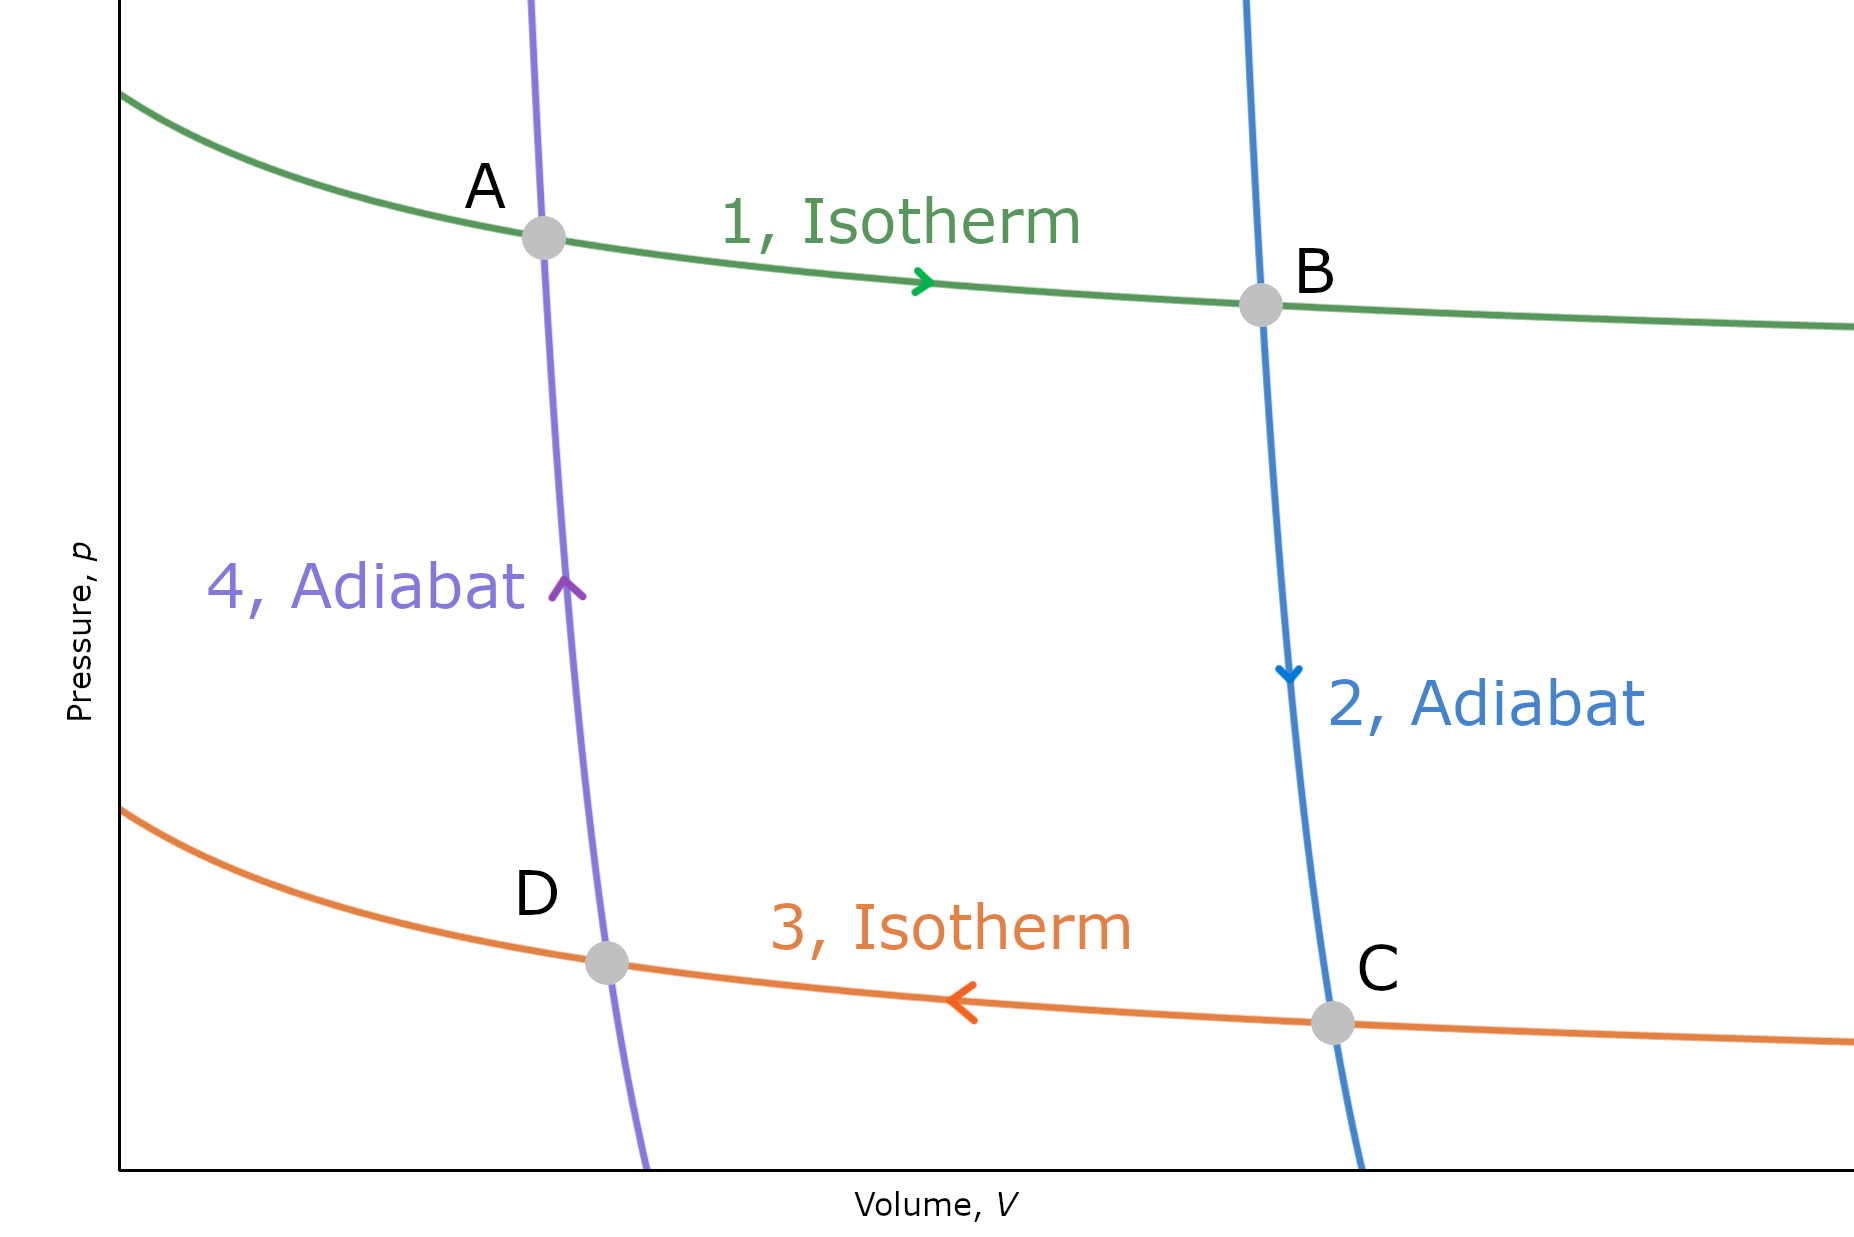
\includegraphics[scale=2]{Images/CarnotCycle.png}
            \caption{Carnot 순환}\label{f4}
        \end{figure}
        따라서 $\displaystyle\oint \difform S = \frac{q_h}{T_h} + \frac{q_c}{T_c}$이다. 이때 과정을 압력-부피 그래프로 나타내면 Figure \ref{f4}와 같다.
        \par 이때 1번과 3번 과정은 등온 과정이므로, $\displaystyle q_h = nRT_h \ln{\frac{V_B}{V_A}}$와 $\displaystyle q_c = nRT_c \ln{\frac{V_D}{V_C}}$를 만족한다. 
        또한, 2번과 4번 과정은 단열 과정이므로 4번 과정에서 $\displaystyle V_A {T_h}^c = V_D {T_c}^c$가, 
        2번 과정에서 $\displaystyle V_B {T_h}^c = V_C {T_c}^c$를 만족한다. 이 둘을 곱하면 다음을 만족한다:
        \begin{equation*}
            V_A V_C {T_h}^c {T_c}^c = V_B V_D {T_h}^c {T_c}^c
        \end{equation*}
        따라서 $\displaystyle V_D / V_C = V_A / V_B$를 만족한다. 따라서 다음을 만족한다:
        \begin{equation*}
            q_c = nRT_c \ln{\frac{V_D}{V_C}} = nRT_c \ln{\frac{V_A}{V_B}} = -nRT_c \ln{\frac{V_B}{V_A}}
        \end{equation*}
        따라서 
        \begin{obs}\label{carnotc}
        \begin{equation*}
            \frac{q_h}{q_c} = -\frac{nRT_h \ln{V_B / V_A}}{-nRT_c \ln{V_B / V_A}} = -\frac{T_h}{T_c}
        \end{equation*}
        \end{obs}
        이므로,
        \begin{equation*}
            \frac{q_h}{T_h} + \frac{q_c}{T_c} = 0
        \end{equation*}
        을 만족한다. 따라서 Carnot 순환에서 $\oint \difform S = 0$을 만족한다. 
        \end{proof}
        \par 열기관의 \textbf{효율(Efficiency, $\eta$)}는 다음과 같이 정의된다:
        \begin{defn}[열기관의 효율]
        \begin{equation*}
            \eta = \frac{\left\vert w \right\vert}{\left\vert q_h \right\vert}
        \end{equation*}
        \end{defn}
        이때 $w$는 열기관이 한 일, $q_h$는 고열원에서 흡수한 열에너지이다. 열기관이 고열원에서 흡수한 열에너지는 일과 저열원으로 방출한 열에너지로 전환되므로, 
        \begin{equation*}
            \eta = \frac{\left\vert q_h \right\vert - \left\vert q_c \right\vert}{\left\vert q_h \right\vert} = 1 - \frac{\left\vert q_c \right\vert}{\left\vert q_h \right\vert}
        \end{equation*}
        로도 쓸 수 있다. Carnot 순환을 하는 열기관에서는 등식 \ref{carnotc}에 의해
        \begin{obs}[Carnot 순환을 하는 열기관의 효율]
        \begin{equation*}
            \eta = 1 - \frac{T_c}{T_h}
        \end{equation*}
        \end{obs}
        로 표현할 수 있다.
        \par 열역학 제2 법칙에 의해, \textit{모든 가역적 열기관은 같은 효율을 가진다.} 
        \begin{proof}
        고열원에서 열에너지를 받아 일을 하는 가역적 열기관 A와 
        저열원에서 열에너지를 받고 A로부터 일을 받아 고열원으로 열에너지를 방출하는 가역적 열기관 B를 가정한다. 이때 A의 효율이 더 높다고 가정하면, '남는 일'이 존재하게 
        된다. 따라서 이 경우 고열원에서 받은 열에너지와 저열원으로 방출하는 열에너지의 차를 모두 '남는 일'로 전환하는 열기관이 된다. 이는 열역학 제2 법칙에 모순이므로, 
        모든 가역적 열기관은 같은 효율을 가진다고 할 수 있다.
        \end{proof}
        \par 모든 열역학 과정은 여러 Carnot 순환의 합으로 근사할 수 있다. 따라서 엔트로피는 상태함수임을 확인할 수 있다.
        \par 온도 $T_h$인 고열원에서 효율 $\eta$의 일을 하고 온도 $T$인 저열원으로 열을 방출하는 가역적 열기관은 다음과 같은 등식을 만족한다:
        \begin{equation*}
            T = \left( 1- \eta\right)T_h
        \end{equation*}
        이를 통해 \textbf{열역학적 온도(Thermodynamic temperature scale)}를 정의할 수 있고, 단위는 K(켈빈, Kelvin)이다.\footnote[11]{%
        2019년에 "Boltzmann 상수를 $1.380\,649 \times 10^{-23}$ J K$^{-1}$로 한다."로 정의되었다.}
        \par 내부 에너지로부터, $\difform U = \difform q + \difform w = \difform q_\mathrm{rev} + \difform w_\mathrm{rev}$ 이므로 
        $\difform q_\mathrm{rev} - \difform q = \difform w - \difform w_\mathrm{rev}$임을 확인할 수 있다. 이때 
        $\difform w - \difform w_\mathrm{rev} \geq 0$이므로, $\difform q_\mathrm{rev} - \difform q \geq 0$이다. 따라서 
        $\displaystyle \difform q_\mathrm{rev} \geq \difform q$이다. 따라서 다음 부등식을 만족한다(\textbf{Clausius 부등식(Clausius inequality)}):
        \begin{law}[Clausius 부등식]\label{clausiusineq}
        \begin{equation*}
            \difform S \geq \frac{\difform q}{T}
        \end{equation*}
        \end{law}
        고립계에서 $\difform q = 0$이므로, \textbf{고립계에서 자발적 변화가 일어날 때 엔트로피는 감소하지 않는다.} 또한, 총 엔트로피에 대해 
        $\difform S_\mathrm{tot} = \difform S + \difform S_\mathrm{sur} \geq 0$을 만족한다. 이때 $\difform S_\mathrm{tot} > 0$, 즉 
        자발적 과정일 때 이는 비가역적 과정이다. 또한, $\difform S_\mathrm{tot} = 0$, 즉 가역적 과정일 때에는 평형 상태에 있다.
        \par 고열원에서 저열원으로 열이 흐르는 과정에서,
        \begin{equation*}
            \difform S \geq \frac{\difform q_h}{T_h} + \frac{\difform q_c}{T_c}
        \end{equation*}
        를 만족한다. 따라서 $\displaystyle\difform q_h = -\difform q_c$이므로,
        \begin{equation*}
            \difform S \geq \left( \frac{1}{T_c} - \frac{1}{T_h} \right)\difform q_c > 0
        \end{equation*}
        을 만족한다. 따라서 열이 온도가 높은 곳에서 온도가 낮은 곳으로 흐르는 것은 자연스럽다.
    \section{열역학 과정에서의 엔트로피 변화}
        \hspace{\parindent} 만약 이상 기체에서 등온 팽창이 가역적으로 일어난다면, $\displaystyle\Delta S = nR \ln{\frac{V_f}{V_i}}$임을 보였다. 또한 가역 과정이므로, $\Delta S_\mathrm{tot} = 0$에서 
        $\displaystyle\Delta S = -nR \ln{\frac{V_f}{V_i}}$임을 보일 수 있다. 만약 등온 팽창이 자유 팽창으로 일어난다면($p_\mathrm{ex} = 0$), $w=0$이고 $\Delta U = 0$에서 
        $q=0$, 즉 $\Delta S_\mathrm{sur} = 0$이다. 따라서 총 엔트로피 변화량은 $\displaystyle\Delta S_\mathrm{tot} = nR \ln{\frac{V_f}{V_i}}$이다. 
        이 또한 $\Delta S > 0$을 만족하고, 따라서 비가역 과정임을 알 수 있다.
        \par 상태 변화에서 또한 엔트로피 변화를 측정할 수 있다. \textbf{정상 상태 변화 온도(Normal transition temperature, $T_\mathrm{trs}$)}는 두 상이 1 atm에서 
        평형을 이루는 온도이다. 이때 $q = \Delta_{\mathrm{trs}}H$이므로, 몰 엔트로피 변화는 다음과 같이 정의된다: 
        \begin{defn}[상태 변화의 몰 엔트로피 변화]\label{trsentr}
        \begin{equation*}
            \Delta_{\mathrm{trs}}S = \frac{\Delta_\mathrm{trs}H}{T_\mathrm{trs}}
        \end{equation*}
        \end{defn}
        만약 상태 변화가 발열 반응일 경우, $\Delta S < 0$이고 흡열 반응일 경우 $\Delta S > 0$이다. 다만 이 경우 $\Delta S_\mathrm{sur}$의 부호는 $\Delta S$의 부호와 
        반대이다. $T_\mathrm{trs}$에서, $\Delta S_\mathrm{tot} = 0$이다. 기화 엔트로피 $\Delta_\mathrm{vap}S^{\circlehbar} \approx 85$ J K$^{-1}$ mol$^{-1}$이다. 
        이를 \textbf{Trouton의 법칙(Trouton's rule)}이라 부르며, 이는 경험적으로 얻어진다. 이는 기화 시에 부피 변화가 물질에 상관없이 비슷하기 때문이라고 설명한다. 
        그러나 여기에서 벗어나는 경우도 존재하는데, 이는 분자 간 인력이 크기 때문에 액체 상태에서 분자의 부분적인 '질서도'가 있기 때문이라고 설명한다.
        \par 엔트로피의 정의에 따라, $\displaystyle S\left(T_f\right) = S\left(T_i\right) + \int_{T_i}^{T_f}\frac{\difform q_\mathrm{rev}}{T}$가 성립하고, 등압 조건에서 
        $\difform q_\mathrm{rev} = \difform H$가 성립하므로 $\difform H = C_p \difform T$에서 다음이 성립한다:
        \begin{cor}[등압 조건에서의 엔트로피]\label{entisobar}
        \begin{equation*}
            S\left(T_f\right) = S\left(T_i\right)+\int_{T_i}^{T_f}\frac{C_p\difform T}{T}
        \end{equation*}
        \end{cor}
        만약 $C_p$가 온도에 무관하다면, 
        \begin{equation*}
            S\left(T_f\right)=S\left(T_i\right) + C_p\int_{T_i}^{T_f}\frac{\difform T}{T} = S\left(T_i\right)+C_p \ln{\frac{T_f}{T_i}}
        \end{equation*}
        가 성립한다. 만약 부피가 일정하고 $C_V$가 온도에 무관하다면, 
        \begin{equation*}
            S\left(T_f\right) = S\left(T_i\right) + C_V \ln{\frac{T_f}{T_i}}
        \end{equation*}
        가 성립한다. 경로가 복잡할 경우 여러 경로로 나누어 생각할 수 있다.
    \section{엔트로피의 측정}
        \hspace{\parindent} 엔트로피는 열량계를 통해 측정된 열 출입을 이용하여 계산될 수 있다. 이때 \textbf{표준 엔트로피(Standard entropy, $S^\circlehbar\left(T\right)$)}는 
        이렇게 계산된 순수한 물질의 1 bar일 때의 엔트로피이다. 
        또한, \textbf{표준 몰 엔트로피(Standard molar entropy, $S_{m}^{\circlehbar}\left(T\right)$)}는 이를 물질의 몰수로 나누어 구한다. 
        \par $T=0$에서 열용량을 구하기 어렵기 때문에, 비금속 고체의 경우 열용량이 $T^3$에 비례한다는 \textbf{Debye 외삽(Debye extrapolation)}을 이용할 수 있다. 이는 
        $C_{p,m} = aT^3$으로 열용량을 근사함으로써, 엔트로피를 추정할 수 있게 한다.
        \par 열역학 제3 법칙은 다음과 같이 기술된다:
        \begin{law}[열역학 제3 법칙]
            모든 완전한 결정은 $T=0$일 때 $S=0$이다. 
        \end{law}
        또한, Walther Hermann Nernst는 다음과 같은 이론을 세웠다:
        \begin{thm}[Nernst 열 이론(Nernst heat theorem)]
            모든 물리적/화학적 변화는 절대 온도가 0으로 수렴할수록 그 과정에 참여하는 모든 물질이 완전히 정렬될 때 그 엔트로피 변화가 0으로 수렴한다.
        \end{thm}
        \par 만약 결정의 배열이 달라질 수 있을 경우, 가능한 미시상태의 수는 1보다 커질 수 있다($\displaystyle\mathcal{W}>0$). 따라서 이때 엔트로피는 0이 아닐 수 있는데, 이를 \textbf{잔류 엔트로피(Residual entropy)}라 한다. 
        얼음 결정은 $3.4$ J K$^{-1}$ mol$^{-1}$의 잔류 엔트로피를 가진다.
        \par 열역학 제3 법칙에 의한 엔트로피 변화는 \textbf{제3 법칙 엔트로피(Third-law entropy)}, 또는 \textbf{엔트로피(Entropy)}라 부른다. 
        \textbf{표준 반응 엔트로피(Standard reaction entropy, $\Delta_r S^{\circlehbar}$)}는 다음과 같이 정의된다:
        \begin{defn}[표준 반응 엔트로피]
        \begin{equation*}
            \Delta_r S^{\circlehbar} = \sum_{\textrm{생성물}} \nu S_m^{\circlehbar} - \sum_{\textrm{반응물}} \nu S_m^{\circlehbar}
        \end{equation*}
        \end{defn}
        또는 화학종 J에 대해 다음과 같이 쓸 수 있다:
        \begin{equation*}
            \Delta_r S^{\circlehbar} = \sum_{\mathrm{J}} \nu_{\mathrm{J}}S_m^{\circlehbar}\left(\mathrm{J}\right)
        \end{equation*}
        이온에 대해서는, $S^{\circlehbar}\left(\textrm(H)^{+},\textrm{aq}\right)=0$으로 관습적으로 정의한다.
        \par 식 \ref{entisobar}에 의해, 엔트로피는 온도 의존성을 가진다. 또한 다음과 같이 표현할 수 있다:
        \begin{cor}
        \begin{equation*}
            \Delta_r S^{\circlehbar}\left(T_2\right) = \Delta_r S^{\circlehbar}\left(T_1 \right)+\int_{T_1}^{T_2}\frac{\Delta_r C_p^{\circlehbar}}{T}\difform T
        \end{equation*}
        \end{cor}
        이때 $\displaystyle\Delta_r C_p^{\circlehbar} = \sum_{\mathrm{J}}\nu_\mathrm{J}C_{p,m}^{\circlehbar}\left(\mathrm{J}\right)$로 정의된다. 이는 Kirchhoff의 법칙(식 \ref{kirlaw})과 
        유사하다. 만약 $\Delta_r C_p^{\circlehbar}$가 온도에 무관하다면, 다음이 성립한다:
        \begin{equation*}
            \Delta_r S^{\circlehbar}\left(T_2\right) = \Delta_r S^{\circlehbar}\left(T_1\right) + \Delta_r C_p^{\circlehbar} \ln{\frac{T_2}{T_1}}
        \end{equation*}
    \section{계에서만 생각하기}\label{ch3sub4}
        \hspace{\parindent} 엔트로피를 계의 상태를 나타내는 변수들로만 나타내기 위해, \textbf{Helmholtz 에너지(Helmholtz energy)}와 \textbf{Gibbs 에너지(Gibbs energy)}라는 새로운 
        에너지를 도입한다. 이는 Clausius 부등식(\ref{clausiusineq})으로부터 출발한다:
        \begin{equation*}
            \difform S - \frac{\difform q}{T} \geq 0
        \end{equation*}
        등적 과정을 가정하면, $\difform q_V = \difform U$가 되어 다음을 만족한다:
        \begin{equation*}
            \difform S - \frac{\difform U}{T} \geq 0
        \end{equation*}
        엔트로피와 내부 에너지 모두 상태 함수이므로, 다음을 만족한다:
        \begin{cor}\label{helmspon}
        \begin{equation*}
            T \difform S \geq \difform U
        \end{equation*}
        \end{cor}
        한편 등압 과정을 가정하면, $\difform q_p = \difform H$를 만족하므로 마찬가지로 다음을 만족한다:
        \begin{cor}\label{gibbspon}
        \begin{equation*}
            T \difform S \geq \difform H
        \end{equation*}
        \end{cor}
        이를 다루기 위해 \textbf{Helmholtz 에너지, $A$}를 다음과 같이 정의한다:
        \begin{defn}[Helmholtz 에너지]
        \begin{equation*}
            A = U - TS
        \end{equation*}
        \end{defn}
        또한, \textbf{Gibbs 에너지, $G$}를 다음과 같이 정의한다:
        \begin{defn}[Gibbs 에너지]
        \begin{equation*}
            G = H - TS
        \end{equation*}
        \end{defn}
        \par 식 \ref{helmspon}을 만족하기 위해서는 $\difform A_{T,V} \leq 0$을, 식 \ref{gibbspon}을 만족하기 위해서는 $\difform G_{T,V} \leq 0$을 만족해야 한다. 
        이때 Helmholtz 에너지는 등온 조건에서 계가 할 수 있는 최대 일에 해당한다. 이는 다음과 같이 증명된다:
        \begin{proof}
        \par $\difform U = \difform q + \difform w$에서, Clausius 부등식 (\ref{clausiusineq})으로부터 $\difform S \geq \difform q/T$를 취하면,
        $\difform U \leq T\difform S + \difform w$를 만족한다. 따라서 $\difform w \geq \difform U -T\difform S$를 만족하고, 따라서 다음을 만족한다:
        \begin{equation*}
            \difform w_{\mathrm{max}} = \difform U - T \difform S
        \end{equation*}
        따라서 등온 조건에서 다음을 만족한다:
        \begin{equation*}
            \difform w_\mathrm{max} = \difform A
        \end{equation*}
        \end{proof}
        마찬가지로, Gibbs 에너지는 등온·등압 조건에서 최대 \textbf{추가 일(Additional work)}에 해당한다. 이는 $\difform G = \difform q + \difform w + \difform \left(pV\right) - T\difform S$라는 
        사실과 $\difform w_\mathrm{rev} = -p\difform V + \difform w_\mathrm{add,max}$라는 사실로부터 유도된다.
        \par \textbf{표준 반응 Gibbs 에너지(Standard Gibbs energy of reaction)}는 다음과 같이 정의된다:
        \begin{defn}[표준 반응 Gibbs 에너지]
        \begin{equation*}
            \Delta_r G^{\circlehbar} = \Delta_r G^\circlehbar - T\Delta_r S^\circlehbar
        \end{equation*}
        \end{defn}
        또한, \textbf{표준 생성 Gibbs 에너지(Standard Gibbs energy of formation, $\Delta_r G^\circlehbar$)}는 표준 상태의 원소로부터 그 화학종이 생성될 때의 표준 반응 Gibbs 에너지에 해당한다. 엔탈피에서와 
        마찬가지로, 표준 반응 Gibbs 에너지는 다음과 같이 쓸 수 있다:
        \begin{defn}[표준 반응 Gibbs 에너지]
        \begin{equation*}
            \Delta_r G^\circlehbar = \sum_{\mathrm{J}}\nu_\mathrm{J}\Delta_f G^\circlehbar\left(\mathrm{J}\right)
        \end{equation*}
        \end{defn}
        이온의 경우, $\displaystyle\Delta_f G^\circlehbar \left(H^{+},\mathrm{aq}\right) = 0$으로 정의한다.
        \par 이온의 용매화 Gibbs 에너지는 \textbf{Born 방정식(Born equation)}으로 추정할 수 있다:
        \begin{law}[Born 방정식]
        \begin{equation*}
            \Delta_\mathrm{solv}G^\circlehbar = -\frac{{z_i}^2 e^2 N_A}{8 \pi \varepsilon_0 r_i}\left( 1-\frac{1}{\epsilon_r}\right)
        \end{equation*}
        \end{law}
        이는 개별 이온을 구형으로 간주하고 수화 반지름 $r_i$와 이온의 전하량 $z_i$, 용매의 비유전율 $\varepsilon_r$에 대해 전기 퍼텐셜을 계산한 것이다.
    \section{열역학 제1 법칙과 제2 법칙을 합친다면?}\label{dudhdadg}
        내부 에너지의 Legendre 변환(Legendre transformation)으로부터 다음 네 개의 식이 성립한다:
        \begin{table}[H]
        \centering
            \begin{tabular}{ c c c }
                \hline
                \rowcolor{lightgray}
                상태함수& &식\\
                \hline
                $\difform U$ & $=$ & $T \difform S - p\difform V$ \\
                $\difform H$ & $=$ & $T \difform S + V\difform p$ \\
                $\difform A$ & $=$ & $-p \difform V - S \difform T$ \\
                $\difform G$ & $=$ & $V\difform p - S \difform T$ \\
                \hline
            \end{tabular}
        \end{table}
        위 식 네 개는 완전미분(\ref{exactdiff} 참고)이므로, 다음 \textbf{Maxwell 관계(Maxwell relation)}가 성립한다:
        \begin{table}[H]
        \centering
            \begin{tabular}{ c|c c c }
                \hline
                \rowcolor{lightgray}
                상태함수& &식& \\
                \hline
                $U$ & $\displaystyle \left(\frac{\partial T}{\partial V}\right)_S$ & $\displaystyle =$ & $\displaystyle -\left(\frac{\partial p}{\partial S}\right)_V$ \\
                $H$ & $\displaystyle \left(\frac{\partial T}{\partial p}\right)_S$ & $\displaystyle =$ & $\displaystyle \left(\frac{\partial V}{\partial S}\right)_p$ \\
                $A$ & $\displaystyle \left(\frac{\partial p}{\partial T}\right)_V$ & $\displaystyle =$ & $\displaystyle \left(\frac{\partial S}{\partial V}\right)_T$ \\
                $G$ & $\displaystyle \left(\frac{\partial V}{\partial T}\right)_p$ & $\displaystyle =$ & $\displaystyle -\left(\frac{\partial S}{\partial p}\right)_T$ \\
                \hline
            \end{tabular}
        \end{table}
        이를 이용하면 내부 압력 $\pi_T = \left(\frac{\partial U}{\partial V}\right)_T$가 다음과 같음을 보일 수 있다:
        \begin{equation*}
            \begin{aligned}
                \pi_T &= \left(\frac{\partial U}{\partial V}\right)_T\\
                &= \left(\frac{\partial U}{\partial S}\right)_V \left(\frac{\partial S}{\partial V}\right)_T + \left(\frac{\partial U}{\partial V}\right)_S\\
                &= T\left(\frac{\partial S}{\partial V}\right)_T -p\\
                &= T\left(\frac{\partial p}{\partial T}\right)_V -p
            \end{aligned}
        \end{equation*}
        \par Gibbs 에너지에서 다음 두 식이 성립한다:
        \begin{cor}\label{gibbspartial}
        \begin{align*}
            \left(\frac{\partial G}{\partial T}\right)_p &= -S\\
            \left(\frac{\partial G}{\partial p}\right)_T &= V
        \end{align*}
        \end{cor}
        \par 또한, Gibbs 에너지의 정의($G = H - TS$)에서 다음이 성립한다:
        \begin{equation*}
            \left(\frac{\partial G}{\partial T}\right)_p = \frac{G-H}{T}
        \end{equation*}
        이때 다음이 성립한다:
        \begin{equation*}
            \begin{aligned}
                \left(\frac{\partial G/T}{\partial T}\right)_p &= \frac{1}{T}\left(\frac{\partial G}{\partial T}\right)_p -\frac{G}{T^2} \\
                &= \frac{G-H}{T^2}-\frac{G}{T^2} = -\frac{H}{T^2}
            \end{aligned}
        \end{equation*}
        따라서 다음 \textbf{Gibbs-Helmholtz 방정식(Gibbs-Helmholtz equation)}이 성립한다:
        \begin{law}[Gibbs-Helmholtz 방정식]\label{gheqn}
        \begin{equation*}
            \left(\frac{\partial G/T}{\partial T}\right)_p = -\frac{H}{T^2}
        \end{equation*}
        \end{law}
        이는 다음과 같이 쓸 수 있다:
        \begin{cor}
        \begin{equation*}
            \left(\frac{\partial \Delta G/T}{\partial T}\right)_p = -\frac{\Delta H}{T^2}
        \end{equation*}
        \end{cor}
        \par 등온 과정에서, Gibbs 에너지는 다음과 같은 식을 만족한다:
        \begin{equation*}
            G_m\left(p_f\right) = G_m\left(p_i\right)+\int_{p_i}^{p_f}V_m \difform p
        \end{equation*}
        만약 이상 기체일 경우, $V_m = RT/p$에서 다음이 성립한다:
        \begin{equation*}
            \begin{aligned}
                G_m\left(p\right) &= G_m^{\circlehbar} + RT \int_{p^\circlehbar}^{p}\frac{1}{p}\difform p\\
                &= G_m^\circlehbar + RT \ln{\frac{p}{p^\circlehbar}}
            \end{aligned}
        \end{equation*}